\documentclass[twoside]{book}

% Packages required by doxygen
\usepackage{fixltx2e}
\usepackage{calc}
\usepackage{doxygen}
\usepackage[export]{adjustbox} % also loads graphicx
\usepackage{graphicx}
\usepackage[utf8]{inputenc}
\usepackage{makeidx}
\usepackage{multicol}
\usepackage{multirow}
\PassOptionsToPackage{warn}{textcomp}
\usepackage{textcomp}
\usepackage[nointegrals]{wasysym}
\usepackage[table]{xcolor}

% Font selection
\usepackage[T1]{fontenc}
\usepackage[scaled=.90]{helvet}
\usepackage{courier}
\usepackage{amssymb}
\usepackage{sectsty}
\renewcommand{\familydefault}{\sfdefault}
\allsectionsfont{%
  \fontseries{bc}\selectfont%
  \color{darkgray}%
}
\renewcommand{\DoxyLabelFont}{%
  \fontseries{bc}\selectfont%
  \color{darkgray}%
}
\newcommand{\+}{\discretionary{\mbox{\scriptsize$\hookleftarrow$}}{}{}}

% Page & text layout
\usepackage{geometry}
\geometry{%
  a4paper,%
  top=2.5cm,%
  bottom=2.5cm,%
  left=2.5cm,%
  right=2.5cm%
}
\tolerance=750
\hfuzz=15pt
\hbadness=750
\setlength{\emergencystretch}{15pt}
\setlength{\parindent}{0cm}
\setlength{\parskip}{3ex plus 2ex minus 2ex}
\makeatletter
\renewcommand{\paragraph}{%
  \@startsection{paragraph}{4}{0ex}{-1.0ex}{1.0ex}{%
    \normalfont\normalsize\bfseries\SS@parafont%
  }%
}
\renewcommand{\subparagraph}{%
  \@startsection{subparagraph}{5}{0ex}{-1.0ex}{1.0ex}{%
    \normalfont\normalsize\bfseries\SS@subparafont%
  }%
}
\makeatother

% Headers & footers
\usepackage{fancyhdr}
\pagestyle{fancyplain}
\fancyhead[LE]{\fancyplain{}{\bfseries\thepage}}
\fancyhead[CE]{\fancyplain{}{}}
\fancyhead[RE]{\fancyplain{}{\bfseries\leftmark}}
\fancyhead[LO]{\fancyplain{}{\bfseries\rightmark}}
\fancyhead[CO]{\fancyplain{}{}}
\fancyhead[RO]{\fancyplain{}{\bfseries\thepage}}
\fancyfoot[LE]{\fancyplain{}{}}
\fancyfoot[CE]{\fancyplain{}{}}
\fancyfoot[RE]{\fancyplain{}{\bfseries\scriptsize Generated by Doxygen }}
\fancyfoot[LO]{\fancyplain{}{\bfseries\scriptsize Generated by Doxygen }}
\fancyfoot[CO]{\fancyplain{}{}}
\fancyfoot[RO]{\fancyplain{}{}}
\renewcommand{\footrulewidth}{0.4pt}
\renewcommand{\chaptermark}[1]{%
  \markboth{#1}{}%
}
\renewcommand{\sectionmark}[1]{%
  \markright{\thesection\ #1}%
}

% Indices & bibliography
\usepackage{natbib}
\usepackage[titles]{tocloft}
\setcounter{tocdepth}{3}
\setcounter{secnumdepth}{5}
\makeindex

% Hyperlinks (required, but should be loaded last)
\usepackage{ifpdf}
\ifpdf
  \usepackage[pdftex,pagebackref=true]{hyperref}
\else
  \usepackage[ps2pdf,pagebackref=true]{hyperref}
\fi
\hypersetup{%
  colorlinks=true,%
  linkcolor=blue,%
  citecolor=blue,%
  unicode%
}

% Custom commands
\newcommand{\clearemptydoublepage}{%
  \newpage{\pagestyle{empty}\cleardoublepage}%
}

\usepackage{caption}
\captionsetup{labelsep=space,justification=centering,font={bf},singlelinecheck=off,skip=4pt,position=top}

%===== C O N T E N T S =====

\begin{document}

% Titlepage & ToC
\hypersetup{pageanchor=false,
             bookmarksnumbered=true,
             pdfencoding=unicode
            }
\pagenumbering{roman}
\begin{titlepage}
\vspace*{7cm}
\begin{center}%
{\Large My Project }\\
\vspace*{1cm}
{\large Generated by Doxygen 1.8.11}\\
\end{center}
\end{titlepage}
\clearemptydoublepage
\tableofcontents
\clearemptydoublepage
\pagenumbering{arabic}
\hypersetup{pageanchor=true}

%--- Begin generated contents ---
\chapter{S\+IR}
\label{md_README}
\hypertarget{md_README}{}
Standard Incident Reporter; simple logging to file, debug and stdout/stderr

\begin{quote}
N\+O\+TE\+: This code is ancient; I wrote it in 2003. It may not compile at all. I have placed it here for posterity. \end{quote}


\subsection*{Description}

Sir is a cross-\/platform A\+N\+SI C library that provides developers with much needed, usually repetitive functionality. Any application of moderate size or complexity requires program output to be sent to various locations, namely the console, log files, a debug window, or G\+UI. Writing the code to do this is painfully repetitious. Enter Sir.

By adding sir to your application\textquotesingle{}s code base, you can perform information output tasks in no time flat. Sir provides functionality that allows you to easily send formatted output to one or more of these destinations simultaneously with one function call\+:


\begin{DoxyItemize}
\item stdout/stderr
\item Log files
\item Callback functions
\item Debug (Windows)
\end{DoxyItemize}

Sir has the capability to prepend output with a standard format timestamp (time()/ctime()), and append carriage return/line feed. Also, Sir may be implemented in C++ applications.

\subsubsection*{Types and return values}

Sir uses the type T\+C\+H\+AR frequently. This type is simply either an 8-\/bit character when the program being built is A\+N\+SI, or a 16-\/bit character when the program is in U\+N\+I\+C\+O\+DE mode. In addition, Sir makes use of the macro \+\_\+T, which, on Windows if U\+N\+I\+C\+O\+DE is being used, transforms string literals to L\char`\"{}\+String\char`\"{}. If you\textquotesingle{}re not using Sir on Windows, you do not need to worry about the \+\_\+T macro.

All Sir functions return type int unless otherwise specified. The success code is zero, and if an error occurs, -\/1 will be returned.

\subsubsection*{Implementation}

Implementing Sir in your application is extremely easy. I have provided it in various forms, including source code, compiled static libraries (debug/release, A\+N\+S\+I/\+U\+N\+I\+C\+O\+DE builds), and a makefile for a shared library. The following section will show example usage.

\#\#\# Example 
\begin{DoxyCode}
\textcolor{preprocessor}{#include "\hyperlink{sir_8h}{sir.h}"}

\textcolor{comment}{/*}
\textcolor{comment}{  Sir type callback function}
\textcolor{comment}{*/}
\textcolor{keywordtype}{void} SirCallback(TCHAR *out, u\_long data);

\textcolor{keywordtype}{int} main(\textcolor{keywordtype}{int} argc, TCHAR *argv[]) \{
  \hyperlink{structsirinit}{sirinit} ss = \{0\}; \textcolor{comment}{/* Declare the Sir initialization structure */}

\textcolor{comment}{/*}
\textcolor{comment}{  Output of types SIRL\_LOG and SIRT\_WARNING}
\textcolor{comment}{  will be sent to stdout.}
\textcolor{comment}{ */}
  ss.f\_stdout = SIRL\_LOG | SIRT\_WARNING;

\textcolor{comment}{/*}
\textcolor{comment}{  Output of type SIRL\_WARNING will be sent}
\textcolor{comment}{  to debug.}
\textcolor{comment}{ */}
  ss.f\_debug = SIRT\_WARNING;

\textcolor{comment}{/*}
\textcolor{comment}{  Output of types SIRL\_ERROR and SIRT\_CRIT}
\textcolor{comment}{  will be sent to stderr.}
\textcolor{comment}{ */}
  ss.f\_stderr = \hyperlink{sir_8h_a06fc87d81c62e9abb8790b6e5713c55ba9c687f088db1de838ea5d5f8a8beed76}{SIRL\_ERROR} | SIRT\_CRIT;

\textcolor{comment}{/*}
\textcolor{comment}{  Set the option bits (Sir.h);}
\textcolor{comment}{  SIRO\_CRLF = \(\backslash\)r\(\backslash\)n will be appended to output,}
\textcolor{comment}{  SIRO\_TIMESTAMP = Time will be prepended to output,}
\textcolor{comment}{  SIRO\_FILES = Sir will handle file output,}
\textcolor{comment}{  SIRO\_CALLBACKS = Sir will handle callback output}
\textcolor{comment}{ */}
  ss.opts = SIRO\_CRLF | SIRO\_TIMESTAMP | SIRO\_FILES | SIRO\_CALLBACKS;

\textcolor{comment}{/*}
\textcolor{comment}{  Initialize the Sir system.}
\textcolor{comment}{ */}

  \textcolor{keywordflow}{if}(0 != Sir\_Init(&ss)) \{
    printf(\textcolor{stringliteral}{"Failed to initialize the Sir system!\(\backslash\)n"});
    \textcolor{keywordflow}{return} 1;
  \} \textcolor{keywordflow}{else} \{
    printf(\textcolor{stringliteral}{"Successfully initialized the Sir system.\(\backslash\)n"});
  \}

\textcolor{comment}{/*}
\textcolor{comment}{  Add a file for output of types SIRL\_WARNING and SIRT\_LOG.}
\textcolor{comment}{ */}
  \textcolor{keywordflow}{if}(0 != Sir\_AddFile(\_T(\textcolor{stringliteral}{"sir.log"}), \hyperlink{sir_8h_a06fc87d81c62e9abb8790b6e5713c55ba1ff2ba86cf1863e3673e5f534e021181}{SIRL\_WARNING} | SIRT\_LOG)) \{
    printf(\textcolor{stringliteral}{"Failed to add file to Sir system!\(\backslash\)n"});
  \} \textcolor{keywordflow}{else} \{
    printf(\textcolor{stringliteral}{"Successfully associated 'sir.log' with SIRT\_WARNING"}
           \textcolor{stringliteral}{" and SIRL\_LOG output types.\(\backslash\)n"});
  \}

\textcolor{comment}{/*}
\textcolor{comment}{  Add a callback for output types of SIRT\_SCREEN.}
\textcolor{comment}{ */}
  \textcolor{keywordflow}{if}(0 != Sir\_AddCallback(SirCallback, SIRL\_SCREEN, 0U)) \{
    printf(\textcolor{stringliteral}{"Failed to add callback to Sir system!\(\backslash\)n"});
  \} \textcolor{keywordflow}{else} \{
    printf(\textcolor{stringliteral}{"Successfully associated SirCallback() with SIRT\_SCREEN"}
           \textcolor{stringliteral}{" output type.\(\backslash\)n"});
  \}

\textcolor{comment}{/*}
\textcolor{comment}{  Send output to all its destinations with one call!}
\textcolor{comment}{ */}

\textcolor{comment}{/*}
\textcolor{comment}{  Sent to all destinations associated with type SIRL\_WARNING or SIRT\_LOG}
\textcolor{comment}{  (or both).}
\textcolor{comment}{ */}
  Sir(\hyperlink{sir_8h_a06fc87d81c62e9abb8790b6e5713c55ba1ff2ba86cf1863e3673e5f534e021181}{SIRL\_WARNING} | SIRT\_LOG, \_T(\textcolor{stringliteral}{"This is a test of the Sir system. This is"})
      \_T(\textcolor{stringliteral}{" only a test. %d, %d, %d"}), 1, 2, 3);

\textcolor{comment}{/*}
\textcolor{comment}{  Sent to all destinations associated with type SIRL\_ERROR or SIRT\_SCREEN}
\textcolor{comment}{  (or both).}
\textcolor{comment}{ */}
  Sir(\hyperlink{sir_8h_a06fc87d81c62e9abb8790b6e5713c55ba9c687f088db1de838ea5d5f8a8beed76}{SIRL\_ERROR} | SIRT\_SCREEN, \_T(\textcolor{stringliteral}{"This is a continuation of the Sir system"})
      \_T(\textcolor{stringliteral}{" test."}));

\textcolor{comment}{/*}
\textcolor{comment}{  Remove the file and callback (disassociates them with output types).}
\textcolor{comment}{ */}
  Sir\_RemFile(\_T(\textcolor{stringliteral}{"sir.log"}));

  Sir\_RemCallback (SirCallback);

\textcolor{comment}{/*}
\textcolor{comment}{  Free allocated resources and reset}
\textcolor{comment}{  the system's state}
\textcolor{comment}{ */}

  Sir\_Cleanup ();

  \textcolor{keywordflow}{return} 0;
\}
\end{DoxyCode}


\subsubsection*{Constants}

\paragraph*{Options}


\begin{DoxyItemize}
\item {\ttfamily S\+I\+R\+O\+\_\+\+T\+I\+M\+E\+S\+T\+A\+MP} \+: Output will be prepended with a timestamp.
\item {\ttfamily S\+I\+R\+O\+\_\+\+C\+R\+LF} \+: Output will be appended with a carriage return and line feed.
\item {\ttfamily S\+I\+R\+O\+\_\+\+F\+I\+L\+ES} \+: Enables the use of disk files for output.
\item {\ttfamily S\+I\+R\+O\+\_\+\+C\+A\+L\+L\+B\+A\+C\+KS} \+: Enables the use of callback functions for output.
\item {\ttfamily S\+I\+R\+O\+\_\+\+D\+E\+F\+A\+U\+LT} \+: Functionally equivalent to S\+I\+R\+O\+\_\+\+T\+I\+M\+E\+S\+T\+A\+MP and S\+I\+R\+O\+\_\+\+C\+R\+LF. Sir will use this option if none are specified.
\end{DoxyItemize}

\paragraph*{Logging levels}


\begin{DoxyItemize}
\item {\ttfamily S\+I\+R\+L\+\_\+\+D\+E\+B\+UG} \+: For debugging information.
\item {\ttfamily S\+I\+R\+L\+\_\+\+E\+R\+R\+OR} \+: To report errors (non-\/fatal).
\item {\ttfamily S\+I\+R\+L\+\_\+\+W\+A\+R\+N\+I\+NG} \+: To report warnings or notifications.
\item {\ttfamily S\+I\+R\+L\+\_\+\+C\+R\+IT} \+: To report fatal errors.
\item {\ttfamily S\+I\+R\+L\+\_\+\+L\+OG} \+: For outputting logging data.
\item {\ttfamily S\+I\+R\+L\+\_\+\+S\+C\+R\+E\+EN} \+: For outputting information to the user. 
\end{DoxyItemize}
\chapter{Class Index}
\section{Class List}
Here are the classes, structs, unions and interfaces with brief descriptions\+:\begin{DoxyCompactList}
\item\contentsline{section}{\hyperlink{structsirinit}{sirinit} \\*Initialization data for the library }{\pageref{structsirinit}}{}
\end{DoxyCompactList}

\chapter{File Index}
\section{File List}
Here is a list of all documented files with brief descriptions\+:\begin{DoxyCompactList}
\item\contentsline{section}{\hyperlink{sir_8c}{sir.\+c} \\*Implementation of the Standard Incident Reporter (S\+IR) library }{\pageref{sir_8c}}{}
\item\contentsline{section}{\hyperlink{sir_8h}{sir.\+h} \\*Definitions for the Standard Incident Reporter (S\+IR) library }{\pageref{sir_8h}}{}
\end{DoxyCompactList}

\chapter{Class Documentation}
\hypertarget{structsirbuf}{}\section{sirbuf Struct Reference}
\label{structsirbuf}\index{sirbuf@{sirbuf}}
\subsection*{Public Attributes}
\begin{DoxyCompactItemize}
\item 
sirchar\+\_\+t $\ast$ {\bfseries ptr}\hypertarget{structsirbuf_ae310afa4abdf67dcd5f49f075e86f75b}{}\label{structsirbuf_ae310afa4abdf67dcd5f49f075e86f75b}

\item 
size\+\_\+t {\bfseries size}\hypertarget{structsirbuf_ac893fa822476bbe7e49ed4d3596ea37b}{}\label{structsirbuf_ac893fa822476bbe7e49ed4d3596ea37b}

\end{DoxyCompactItemize}


The documentation for this struct was generated from the following file\+:\begin{DoxyCompactItemize}
\item 
\hyperlink{sir_8h}{sir.\+h}\end{DoxyCompactItemize}

\hypertarget{structsircallback}{}\section{sircallback Struct Reference}
\label{structsircallback}\index{sircallback@{sircallback}}
\subsection*{Public Attributes}
\begin{DoxyCompactItemize}
\item 
\hyperlink{sir_8h_ace3ea4091f07fc8e8cde5b1c14b3fd29}{sircallbackfn} {\bfseries cb}\hypertarget{structsircallback_a3ef42608fdde48df814d21a10b8db417}{}\label{structsircallback_a3ef42608fdde48df814d21a10b8db417}

\item 
sir\+\_\+levels {\bfseries levels}\hypertarget{structsircallback_afe26255fbc47f4337fe51d877d8de82e}{}\label{structsircallback_afe26255fbc47f4337fe51d877d8de82e}

\item 
uint64\+\_\+t {\bfseries data}\hypertarget{structsircallback_a58c143d45ba4a6a38d3e82bdc0fb16ce}{}\label{structsircallback_a58c143d45ba4a6a38d3e82bdc0fb16ce}

\end{DoxyCompactItemize}


The documentation for this struct was generated from the following file\+:\begin{DoxyCompactItemize}
\item 
\hyperlink{sir_8h}{sir.\+h}\end{DoxyCompactItemize}

\hypertarget{structsircallbacks}{}\section{sircallbacks Struct Reference}
\label{structsircallbacks}\index{sircallbacks@{sircallbacks}}


Collaboration diagram for sircallbacks\+:\nopagebreak
\begin{figure}[H]
\begin{center}
\leavevmode
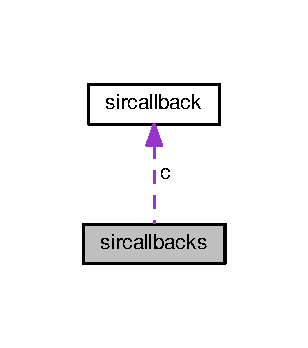
\includegraphics[width=148pt]{structsircallbacks__coll__graph}
\end{center}
\end{figure}
\subsection*{Public Attributes}
\begin{DoxyCompactItemize}
\item 
\hyperlink{structsircallback}{sircallback} $\ast$ {\bfseries c} \mbox{[}\hyperlink{sir_8h_a37364e1ca242c22f3b3d10949f9d78d9}{S\+I\+R\+\_\+\+M\+A\+X\+C\+A\+L\+L\+B\+A\+C\+KS}\mbox{]}\hypertarget{structsircallbacks_a6e31f58637668ff6b9c4829f5a1ac4d7}{}\label{structsircallbacks_a6e31f58637668ff6b9c4829f5a1ac4d7}

\item 
size\+\_\+t {\bfseries count}\hypertarget{structsircallbacks_a2da7cd36b0b3db1ef158a700b4d61f07}{}\label{structsircallbacks_a2da7cd36b0b3db1ef158a700b4d61f07}

\end{DoxyCompactItemize}


The documentation for this struct was generated from the following file\+:\begin{DoxyCompactItemize}
\item 
\hyperlink{sir_8h}{sir.\+h}\end{DoxyCompactItemize}

\hypertarget{structsirfile}{}\section{sirfile Struct Reference}
\label{structsirfile}\index{sirfile@{sirfile}}
\subsection*{Public Attributes}
\begin{DoxyCompactItemize}
\item 
sirchar\+\_\+t $\ast$ {\bfseries path}\hypertarget{structsirfile_a9f4b5f85f13a12175ebcced6820f4257}{}\label{structsirfile_a9f4b5f85f13a12175ebcced6820f4257}

\item 
sir\+\_\+levels {\bfseries levels}\hypertarget{structsirfile_a3485c3a00fd97bb826277b43380fff88}{}\label{structsirfile_a3485c3a00fd97bb826277b43380fff88}

\end{DoxyCompactItemize}


The documentation for this struct was generated from the following file\+:\begin{DoxyCompactItemize}
\item 
\hyperlink{sir_8h}{sir.\+h}\end{DoxyCompactItemize}

\hypertarget{structsirfiles}{}\section{sirfiles Struct Reference}
\label{structsirfiles}\index{sirfiles@{sirfiles}}


Collaboration diagram for sirfiles\+:\nopagebreak
\begin{figure}[H]
\begin{center}
\leavevmode
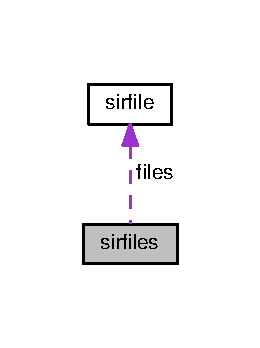
\includegraphics[width=125pt]{structsirfiles__coll__graph}
\end{center}
\end{figure}
\subsection*{Public Attributes}
\begin{DoxyCompactItemize}
\item 
\hyperlink{structsirfile}{sirfile} $\ast$ {\bfseries files} \mbox{[}\hyperlink{sir_8h_aa1080a4bec531adb6d25c87ac4734399}{S\+I\+R\+\_\+\+M\+A\+X\+F\+I\+L\+ES}\mbox{]}\hypertarget{structsirfiles_a65c5e5be7ebd527d2304fc8d6cf30b45}{}\label{structsirfiles_a65c5e5be7ebd527d2304fc8d6cf30b45}

\item 
size\+\_\+t {\bfseries count}\hypertarget{structsirfiles_a021828ca86b408a02dee81fb8e4ade6f}{}\label{structsirfiles_a021828ca86b408a02dee81fb8e4ade6f}

\end{DoxyCompactItemize}


The documentation for this struct was generated from the following file\+:\begin{DoxyCompactItemize}
\item 
\hyperlink{sir_8h}{sir.\+h}\end{DoxyCompactItemize}

\hypertarget{structsirinit}{}\section{sirinit Struct Reference}
\label{structsirinit}\index{sirinit@{sirinit}}


Initialization data for the library.  




{\ttfamily \#include $<$sir.\+h$>$}

\subsection*{Public Attributes}
\begin{DoxyCompactItemize}
\item 
uint32\+\_\+t {\bfseries opts}\hypertarget{structsirinit_a8a16d181e8dde73266d6b6e45e8bd9c0}{}\label{structsirinit_a8a16d181e8dde73266d6b6e45e8bd9c0}

\item 
uint32\+\_\+t {\bfseries f\+\_\+stdout}\hypertarget{structsirinit_a3cd9b91059bd65f1562ba7f6afd40f8c}{}\label{structsirinit_a3cd9b91059bd65f1562ba7f6afd40f8c}

\item 
uint32\+\_\+t {\bfseries f\+\_\+stderr}\hypertarget{structsirinit_a0bcca99abfd9d8b18d62f263187a28b1}{}\label{structsirinit_a0bcca99abfd9d8b18d62f263187a28b1}

\item 
uint32\+\_\+t {\bfseries f\+\_\+debug}\hypertarget{structsirinit_abec44c66fd017d2b572d4b4665e49b27}{}\label{structsirinit_abec44c66fd017d2b572d4b4665e49b27}

\item 
uint32\+\_\+t {\bfseries f\+\_\+syslog}\hypertarget{structsirinit_a12495a5dc6bff02e01274c2eb38ec362}{}\label{structsirinit_a12495a5dc6bff02e01274c2eb38ec362}

\item 
const sirchar\+\_\+t $\ast$ {\bfseries fmt\+Override}\hypertarget{structsirinit_a240e4460d815b73ae7b34e40d4f703f6}{}\label{structsirinit_a240e4460d815b73ae7b34e40d4f703f6}

\item 
const sirchar\+\_\+t $\ast$ {\bfseries app\+Name}\hypertarget{structsirinit_aeb5ae1905f653b2ba48bc46230cfc0cc}{}\label{structsirinit_aeb5ae1905f653b2ba48bc46230cfc0cc}

\end{DoxyCompactItemize}


\subsection{Detailed Description}
Initialization data for the library. 

Allocate an instance of this struct and pass it to \hyperlink{sir_8h_a99c2210334096965d23626fa50dc5d6b}{sir\+\_\+init} in order to begin using the library.

Don\textquotesingle{}t forget to call \hyperlink{sir_8h_ae3d423234ff95592b8d800b8bf092489}{sir\+\_\+cleanup} when you\textquotesingle{}re done. 

The documentation for this struct was generated from the following file\+:\begin{DoxyCompactItemize}
\item 
\hyperlink{sir_8h}{sir.\+h}\end{DoxyCompactItemize}

\chapter{File Documentation}
\doxysection{sir.\+c File Reference}
\hypertarget{sir_8c}{}\label{sir_8c}\index{sir.c@{sir.c}}


Public interface.  


{\ttfamily \#include \"{}sir.\+h\"{}}\newline
{\ttfamily \#include \"{}sirinternal.\+h\"{}}\newline
{\ttfamily \#include \"{}sirfilecache.\+h\"{}}\newline
{\ttfamily \#include \"{}sirtextstyle.\+h\"{}}\newline
{\ttfamily \#include \"{}sirdefaults.\+h\"{}}\newline
\doxysubsubsection*{Functions}
\begin{DoxyCompactItemize}
\item 
bool \mbox{\hyperlink{group__public_gaa4f5707f5e4ed9702cde75a8c80c4e4a}{sir\+\_\+init}} (\mbox{\hyperlink{group__public_structsirinit}{sirinit}} \texorpdfstring{$\ast$}{*}si)
\begin{DoxyCompactList}\small\item\em Initializes libsir. \end{DoxyCompactList}\item 
bool \mbox{\hyperlink{group__public_ga6f17febe99cb0beb6f8119283cc62d42}{sir\+\_\+stdoutlevels}} (\mbox{\hyperlink{group__public_ga7ee5f2908abd2df9e89bcab0b6608edd}{sir\+\_\+levels}} levels)
\begin{DoxyCompactList}\small\item\em Sets levels sent to {\itshape stdout}. \end{DoxyCompactList}\item 
bool \mbox{\hyperlink{group__public_gac117aaf4a045115e58ba4471f9a4747f}{sir\+\_\+stdoutopts}} (\mbox{\hyperlink{group__public_gafb659914aac0129182d86f7d3414e85d}{sir\+\_\+options}} opts)
\begin{DoxyCompactList}\small\item\em Sets formatting options for {\itshape stdout}. \end{DoxyCompactList}\item 
bool \mbox{\hyperlink{group__public_ga421c13f6e269440cef0ac5c1ff3e65dd}{sir\+\_\+stderrlevels}} (\mbox{\hyperlink{group__public_ga7ee5f2908abd2df9e89bcab0b6608edd}{sir\+\_\+levels}} levels)
\begin{DoxyCompactList}\small\item\em Sets levels sent to {\itshape stderr}. \end{DoxyCompactList}\item 
bool \mbox{\hyperlink{group__public_ga0e78fb3ad87f02ef0f056a34200a4ab9}{sir\+\_\+stderropts}} (\mbox{\hyperlink{group__public_gafb659914aac0129182d86f7d3414e85d}{sir\+\_\+options}} opts)
\begin{DoxyCompactList}\small\item\em Sets formatting options for {\itshape stderr}. \end{DoxyCompactList}\item 
bool \mbox{\hyperlink{group__public_ga2b383287c821bb519868776a4d8bae83}{sir\+\_\+sysloglevels}} (\mbox{\hyperlink{group__public_ga7ee5f2908abd2df9e89bcab0b6608edd}{sir\+\_\+levels}} levels)
\begin{DoxyCompactList}\small\item\em Sets levels sent to {\itshape syslog} (if available). \end{DoxyCompactList}\item 
bool \mbox{\hyperlink{group__public_ga2e789c5d4a997d3ad7a528bf7a878936}{sir\+\_\+filelevels}} (\mbox{\hyperlink{group__public_gab8f5ba0bae678457f8bce30e961c9eb6}{sirfileid\+\_\+t}} id, \mbox{\hyperlink{group__public_ga7ee5f2908abd2df9e89bcab0b6608edd}{sir\+\_\+levels}} levels)
\begin{DoxyCompactList}\small\item\em Sets levels sent to a log file. \end{DoxyCompactList}\item 
bool \mbox{\hyperlink{group__public_gaab0821c7a1b10e18e9a68b3e8df6f613}{sir\+\_\+fileopts}} (\mbox{\hyperlink{group__public_gab8f5ba0bae678457f8bce30e961c9eb6}{sirfileid\+\_\+t}} id, \mbox{\hyperlink{group__public_gafb659914aac0129182d86f7d3414e85d}{sir\+\_\+options}} opts)
\begin{DoxyCompactList}\small\item\em Sets formatting options for a log file. \end{DoxyCompactList}\item 
bool \mbox{\hyperlink{group__public_ga9bf3e92cefac01de4e3c6c359a58706f}{sir\+\_\+cleanup}} (void)
\begin{DoxyCompactList}\small\item\em Frees allocated resources and resets internal state. \end{DoxyCompactList}\item 
uint16\+\_\+t \mbox{\hyperlink{group__errors_ga98d098b444b4e8096aad21df81105e74}{sir\+\_\+geterror}} (\mbox{\hyperlink{group__public_ga1d2f790e2dabc69c8a625f2ee5dc583a}{sirchar\+\_\+t}} message\mbox{[}256\mbox{]})
\begin{DoxyCompactList}\small\item\em Retrieves information about the last error that occurred within the context of libsir or lower. \end{DoxyCompactList}\item 
bool \mbox{\hyperlink{group__public_ga3580e004c0c568c225a6d1a1bc5e9ea2}{sir\+\_\+debug}} (const \mbox{\hyperlink{group__public_ga1d2f790e2dabc69c8a625f2ee5dc583a}{sirchar\+\_\+t}} \texorpdfstring{$\ast$}{*}format,...)
\begin{DoxyCompactList}\small\item\em Log a formatted debug-\/level message. \end{DoxyCompactList}\item 
bool \mbox{\hyperlink{group__public_ga707b1de6ceee2e3091b7d4ecf0f8758e}{sir\+\_\+info}} (const \mbox{\hyperlink{group__public_ga1d2f790e2dabc69c8a625f2ee5dc583a}{sirchar\+\_\+t}} \texorpdfstring{$\ast$}{*}format,...)
\begin{DoxyCompactList}\small\item\em Log a formatted informational message. \end{DoxyCompactList}\item 
bool \mbox{\hyperlink{group__public_gab17d7622664c42afaafa66c53542dfeb}{sir\+\_\+notice}} (const \mbox{\hyperlink{group__public_ga1d2f790e2dabc69c8a625f2ee5dc583a}{sirchar\+\_\+t}} \texorpdfstring{$\ast$}{*}format,...)
\begin{DoxyCompactList}\small\item\em Log a formatted notice message. \end{DoxyCompactList}\item 
bool \mbox{\hyperlink{group__public_ga3c4ca38dbb2a5e99e2d862dfdbd6f97a}{sir\+\_\+warn}} (const \mbox{\hyperlink{group__public_ga1d2f790e2dabc69c8a625f2ee5dc583a}{sirchar\+\_\+t}} \texorpdfstring{$\ast$}{*}format,...)
\begin{DoxyCompactList}\small\item\em Log a formatted warning message. \end{DoxyCompactList}\item 
bool \mbox{\hyperlink{group__public_gace667f9ba844f541bc41c61c94ed93f3}{sir\+\_\+error}} (const \mbox{\hyperlink{group__public_ga1d2f790e2dabc69c8a625f2ee5dc583a}{sirchar\+\_\+t}} \texorpdfstring{$\ast$}{*}format,...)
\begin{DoxyCompactList}\small\item\em Log a formatted error message. \end{DoxyCompactList}\item 
bool \mbox{\hyperlink{group__public_ga29cff3ca15309cca61066870674f54c3}{sir\+\_\+crit}} (const \mbox{\hyperlink{group__public_ga1d2f790e2dabc69c8a625f2ee5dc583a}{sirchar\+\_\+t}} \texorpdfstring{$\ast$}{*}format,...)
\begin{DoxyCompactList}\small\item\em Log a formatted critical error message. \end{DoxyCompactList}\item 
bool \mbox{\hyperlink{group__public_ga48e9fb49c28b31a09d48eb0e90468679}{sir\+\_\+alert}} (const \mbox{\hyperlink{group__public_ga1d2f790e2dabc69c8a625f2ee5dc583a}{sirchar\+\_\+t}} \texorpdfstring{$\ast$}{*}format,...)
\begin{DoxyCompactList}\small\item\em Log a formatted alert message. \end{DoxyCompactList}\item 
bool \mbox{\hyperlink{group__public_gabace08a061ddb85494e28bd3a518bb58}{sir\+\_\+emerg}} (const \mbox{\hyperlink{group__public_ga1d2f790e2dabc69c8a625f2ee5dc583a}{sirchar\+\_\+t}} \texorpdfstring{$\ast$}{*}format,...)
\begin{DoxyCompactList}\small\item\em Log a formatted emergency message. \end{DoxyCompactList}\item 
\mbox{\hyperlink{group__public_gab8f5ba0bae678457f8bce30e961c9eb6}{sirfileid\+\_\+t}} \mbox{\hyperlink{group__public_ga4db9ea5b34afaa585f6b9cda84f385e9}{sir\+\_\+addfile}} (const \mbox{\hyperlink{group__public_ga1d2f790e2dabc69c8a625f2ee5dc583a}{sirchar\+\_\+t}} \texorpdfstring{$\ast$}{*}path, \mbox{\hyperlink{group__public_ga7ee5f2908abd2df9e89bcab0b6608edd}{sir\+\_\+levels}} levels, \mbox{\hyperlink{group__public_gafb659914aac0129182d86f7d3414e85d}{sir\+\_\+options}} opts)
\begin{DoxyCompactList}\small\item\em Add a log file to receive formatted output for one or more \doxylink{group__public_ga4a3303c67acd49bea38fd3565d458cb2}{sir\+\_\+level}. \end{DoxyCompactList}\item 
bool \mbox{\hyperlink{group__public_ga4a774bf801d0356b90f29aa69688ef86}{sir\+\_\+remfile}} (\mbox{\hyperlink{group__public_gab8f5ba0bae678457f8bce30e961c9eb6}{sirfileid\+\_\+t}} id)
\begin{DoxyCompactList}\small\item\em Remove a previously added log file. \end{DoxyCompactList}\item 
bool \mbox{\hyperlink{group__public_gaa628fae976081e7aaa302e5c5e43e06c}{sir\+\_\+settextstyle}} (\mbox{\hyperlink{group__public_ga4a3303c67acd49bea38fd3565d458cb2}{sir\+\_\+level}} level, \mbox{\hyperlink{group__public_ga3bd5959a607e5280a8db90ada2d80caf}{sir\+\_\+textstyle}} style)
\begin{DoxyCompactList}\small\item\em Sets the text style in {\itshape stdio} output for a \doxylink{group__public_ga4a3303c67acd49bea38fd3565d458cb2}{sir\+\_\+level} of output. \end{DoxyCompactList}\item 
bool \mbox{\hyperlink{group__public_ga932eec2f9c73eecdd2b6b935452e5eed}{sir\+\_\+resettextstyles}} (void)
\begin{DoxyCompactList}\small\item\em Resets all {\itshape stdio} text styles to their default values. \end{DoxyCompactList}\end{DoxyCompactItemize}


\doxysubsection{Detailed Description}
Public interface. 

This file and accompanying source code originated from \href{https://github.com/aremmell/libsir}{\texttt{ https\+://github.\+com/aremmell/libsir}}. If you obtained it elsewhere, all bets are off.

\begin{DoxyAuthor}{Author}
Ryan M. Lederman \href{mailto:lederman@gmail.com}{\texttt{ lederman@gmail.\+com}} 
\end{DoxyAuthor}
\begin{DoxyVersion}{Version}
2.\+1.\+1 
\end{DoxyVersion}
\begin{DoxyCopyright}{Copyright}

\end{DoxyCopyright}
The MIT License (MIT)

Copyright (c) 2018 Ryan M. Lederman

Permission is hereby granted, free of charge, to any person obtaining a copy of this software and associated documentation files (the \"{}\+Software\"{}), to deal in the Software without restriction, including without limitation the rights to use, copy, modify, merge, publish, distribute, sublicense, and/or sell copies of the Software, and to permit persons to whom the Software is furnished to do so, subject to the following conditions\+:

The above copyright notice and this permission notice shall be included in all copies or substantial portions of the Software.

THE SOFTWARE IS PROVIDED \"{}\+AS IS\"{}, WITHOUT WARRANTY OF ANY KIND, EXPRESS OR IMPLIED, INCLUDING BUT NOT LIMITED TO THE WARRANTIES OF MERCHANTABILITY, FITNESS FOR A PARTICULAR PURPOSE AND NONINFRINGEMENT. IN NO EVENT SHALL THE AUTHORS OR COPYRIGHT HOLDERS BE LIABLE FOR ANY CLAIM, DAMAGES OR OTHER LIABILITY, WHETHER IN AN ACTION OF CONTRACT, TORT OR OTHERWISE, ARISING FROM, OUT OF OR IN CONNECTION WITH THE SOFTWARE OR THE USE OR OTHER DEALINGS IN THE SOFTWARE. 

Definition in file \mbox{\hyperlink{sir_8c_source}{sir.\+c}}.


\doxysection{sir.\+h File Reference}
\hypertarget{sir_8h}{}\label{sir_8h}\index{sir.h@{sir.h}}


Public interface.  


{\ttfamily \#include \"{}sirplatform.\+h\"{}}\newline
{\ttfamily \#include \"{}sirtypes.\+h\"{}}\newline
\doxysubsubsection*{Functions}
\begin{DoxyCompactItemize}
\item 
bool \mbox{\hyperlink{group__public_gaa4f5707f5e4ed9702cde75a8c80c4e4a}{sir\+\_\+init}} (\mbox{\hyperlink{group__public_structsirinit}{sirinit}} \texorpdfstring{$\ast$}{*}si)
\begin{DoxyCompactList}\small\item\em Initializes libsir. \end{DoxyCompactList}\item 
bool \mbox{\hyperlink{group__public_ga6f17febe99cb0beb6f8119283cc62d42}{sir\+\_\+stdoutlevels}} (\mbox{\hyperlink{group__public_ga7ee5f2908abd2df9e89bcab0b6608edd}{sir\+\_\+levels}} levels)
\begin{DoxyCompactList}\small\item\em Sets levels sent to {\itshape stdout}. \end{DoxyCompactList}\item 
bool \mbox{\hyperlink{group__public_gac117aaf4a045115e58ba4471f9a4747f}{sir\+\_\+stdoutopts}} (\mbox{\hyperlink{group__public_gafb659914aac0129182d86f7d3414e85d}{sir\+\_\+options}} opts)
\begin{DoxyCompactList}\small\item\em Sets formatting options for {\itshape stdout}. \end{DoxyCompactList}\item 
bool \mbox{\hyperlink{group__public_ga421c13f6e269440cef0ac5c1ff3e65dd}{sir\+\_\+stderrlevels}} (\mbox{\hyperlink{group__public_ga7ee5f2908abd2df9e89bcab0b6608edd}{sir\+\_\+levels}} levels)
\begin{DoxyCompactList}\small\item\em Sets levels sent to {\itshape stderr}. \end{DoxyCompactList}\item 
bool \mbox{\hyperlink{group__public_ga0e78fb3ad87f02ef0f056a34200a4ab9}{sir\+\_\+stderropts}} (\mbox{\hyperlink{group__public_gafb659914aac0129182d86f7d3414e85d}{sir\+\_\+options}} opts)
\begin{DoxyCompactList}\small\item\em Sets formatting options for {\itshape stderr}. \end{DoxyCompactList}\item 
bool \mbox{\hyperlink{group__public_ga2b383287c821bb519868776a4d8bae83}{sir\+\_\+sysloglevels}} (\mbox{\hyperlink{group__public_ga7ee5f2908abd2df9e89bcab0b6608edd}{sir\+\_\+levels}} levels)
\begin{DoxyCompactList}\small\item\em Sets levels sent to {\itshape syslog} (if available). \end{DoxyCompactList}\item 
bool \mbox{\hyperlink{group__public_ga2e789c5d4a997d3ad7a528bf7a878936}{sir\+\_\+filelevels}} (\mbox{\hyperlink{group__public_gab8f5ba0bae678457f8bce30e961c9eb6}{sirfileid\+\_\+t}} id, \mbox{\hyperlink{group__public_ga7ee5f2908abd2df9e89bcab0b6608edd}{sir\+\_\+levels}} levels)
\begin{DoxyCompactList}\small\item\em Sets levels sent to a log file. \end{DoxyCompactList}\item 
bool \mbox{\hyperlink{group__public_gaab0821c7a1b10e18e9a68b3e8df6f613}{sir\+\_\+fileopts}} (\mbox{\hyperlink{group__public_gab8f5ba0bae678457f8bce30e961c9eb6}{sirfileid\+\_\+t}} id, \mbox{\hyperlink{group__public_gafb659914aac0129182d86f7d3414e85d}{sir\+\_\+options}} opts)
\begin{DoxyCompactList}\small\item\em Sets formatting options for a log file. \end{DoxyCompactList}\item 
bool \mbox{\hyperlink{group__public_ga9bf3e92cefac01de4e3c6c359a58706f}{sir\+\_\+cleanup}} (void)
\begin{DoxyCompactList}\small\item\em Frees allocated resources and resets internal state. \end{DoxyCompactList}\item 
uint16\+\_\+t \mbox{\hyperlink{group__errors_ga98d098b444b4e8096aad21df81105e74}{sir\+\_\+geterror}} (\mbox{\hyperlink{group__public_ga1d2f790e2dabc69c8a625f2ee5dc583a}{sirchar\+\_\+t}} message\mbox{[}256\mbox{]})
\begin{DoxyCompactList}\small\item\em Retrieves information about the last error that occurred within the context of libsir or lower. \end{DoxyCompactList}\item 
bool \mbox{\hyperlink{group__public_ga3580e004c0c568c225a6d1a1bc5e9ea2}{sir\+\_\+debug}} (const \mbox{\hyperlink{group__public_ga1d2f790e2dabc69c8a625f2ee5dc583a}{sirchar\+\_\+t}} \texorpdfstring{$\ast$}{*}format,...)
\begin{DoxyCompactList}\small\item\em Log a formatted debug-\/level message. \end{DoxyCompactList}\item 
bool \mbox{\hyperlink{group__public_ga707b1de6ceee2e3091b7d4ecf0f8758e}{sir\+\_\+info}} (const \mbox{\hyperlink{group__public_ga1d2f790e2dabc69c8a625f2ee5dc583a}{sirchar\+\_\+t}} \texorpdfstring{$\ast$}{*}format,...)
\begin{DoxyCompactList}\small\item\em Log a formatted informational message. \end{DoxyCompactList}\item 
bool \mbox{\hyperlink{group__public_gab17d7622664c42afaafa66c53542dfeb}{sir\+\_\+notice}} (const \mbox{\hyperlink{group__public_ga1d2f790e2dabc69c8a625f2ee5dc583a}{sirchar\+\_\+t}} \texorpdfstring{$\ast$}{*}format,...)
\begin{DoxyCompactList}\small\item\em Log a formatted notice message. \end{DoxyCompactList}\item 
bool \mbox{\hyperlink{group__public_ga3c4ca38dbb2a5e99e2d862dfdbd6f97a}{sir\+\_\+warn}} (const \mbox{\hyperlink{group__public_ga1d2f790e2dabc69c8a625f2ee5dc583a}{sirchar\+\_\+t}} \texorpdfstring{$\ast$}{*}format,...)
\begin{DoxyCompactList}\small\item\em Log a formatted warning message. \end{DoxyCompactList}\item 
bool \mbox{\hyperlink{group__public_gace667f9ba844f541bc41c61c94ed93f3}{sir\+\_\+error}} (const \mbox{\hyperlink{group__public_ga1d2f790e2dabc69c8a625f2ee5dc583a}{sirchar\+\_\+t}} \texorpdfstring{$\ast$}{*}format,...)
\begin{DoxyCompactList}\small\item\em Log a formatted error message. \end{DoxyCompactList}\item 
bool \mbox{\hyperlink{group__public_ga29cff3ca15309cca61066870674f54c3}{sir\+\_\+crit}} (const \mbox{\hyperlink{group__public_ga1d2f790e2dabc69c8a625f2ee5dc583a}{sirchar\+\_\+t}} \texorpdfstring{$\ast$}{*}format,...)
\begin{DoxyCompactList}\small\item\em Log a formatted critical error message. \end{DoxyCompactList}\item 
bool \mbox{\hyperlink{group__public_ga48e9fb49c28b31a09d48eb0e90468679}{sir\+\_\+alert}} (const \mbox{\hyperlink{group__public_ga1d2f790e2dabc69c8a625f2ee5dc583a}{sirchar\+\_\+t}} \texorpdfstring{$\ast$}{*}format,...)
\begin{DoxyCompactList}\small\item\em Log a formatted alert message. \end{DoxyCompactList}\item 
bool \mbox{\hyperlink{group__public_gabace08a061ddb85494e28bd3a518bb58}{sir\+\_\+emerg}} (const \mbox{\hyperlink{group__public_ga1d2f790e2dabc69c8a625f2ee5dc583a}{sirchar\+\_\+t}} \texorpdfstring{$\ast$}{*}format,...)
\begin{DoxyCompactList}\small\item\em Log a formatted emergency message. \end{DoxyCompactList}\item 
\mbox{\hyperlink{group__public_gab8f5ba0bae678457f8bce30e961c9eb6}{sirfileid\+\_\+t}} \mbox{\hyperlink{group__public_ga4db9ea5b34afaa585f6b9cda84f385e9}{sir\+\_\+addfile}} (const \mbox{\hyperlink{group__public_ga1d2f790e2dabc69c8a625f2ee5dc583a}{sirchar\+\_\+t}} \texorpdfstring{$\ast$}{*}path, \mbox{\hyperlink{group__public_ga7ee5f2908abd2df9e89bcab0b6608edd}{sir\+\_\+levels}} levels, \mbox{\hyperlink{group__public_gafb659914aac0129182d86f7d3414e85d}{sir\+\_\+options}} opts)
\begin{DoxyCompactList}\small\item\em Add a log file to receive formatted output for one or more \doxylink{group__public_ga4a3303c67acd49bea38fd3565d458cb2}{sir\+\_\+level}. \end{DoxyCompactList}\item 
bool \mbox{\hyperlink{group__public_ga4a774bf801d0356b90f29aa69688ef86}{sir\+\_\+remfile}} (\mbox{\hyperlink{group__public_gab8f5ba0bae678457f8bce30e961c9eb6}{sirfileid\+\_\+t}} id)
\begin{DoxyCompactList}\small\item\em Remove a previously added log file. \end{DoxyCompactList}\item 
bool \mbox{\hyperlink{group__public_gaa628fae976081e7aaa302e5c5e43e06c}{sir\+\_\+settextstyle}} (\mbox{\hyperlink{group__public_ga4a3303c67acd49bea38fd3565d458cb2}{sir\+\_\+level}} level, \mbox{\hyperlink{group__public_ga3bd5959a607e5280a8db90ada2d80caf}{sir\+\_\+textstyle}} style)
\begin{DoxyCompactList}\small\item\em Sets the text style in {\itshape stdio} output for a \doxylink{group__public_ga4a3303c67acd49bea38fd3565d458cb2}{sir\+\_\+level} of output. \end{DoxyCompactList}\item 
bool \mbox{\hyperlink{group__public_ga932eec2f9c73eecdd2b6b935452e5eed}{sir\+\_\+resettextstyles}} (void)
\begin{DoxyCompactList}\small\item\em Resets all {\itshape stdio} text styles to their default values. \end{DoxyCompactList}\end{DoxyCompactItemize}


\doxysubsection{Detailed Description}
Public interface. 

This file and accompanying source code originated from \href{https://github.com/aremmell/libsir}{\texttt{ https\+://github.\+com/aremmell/libsir}}. If you obtained it elsewhere, all bets are off.

\begin{DoxyAuthor}{Author}
Ryan M. Lederman \href{mailto:lederman@gmail.com}{\texttt{ lederman@gmail.\+com}} 
\end{DoxyAuthor}
\begin{DoxyVersion}{Version}
2.\+1.\+1 
\end{DoxyVersion}
\begin{DoxyCopyright}{Copyright}

\end{DoxyCopyright}
The MIT License (MIT)

Copyright (c) 2018 Ryan M. Lederman

Permission is hereby granted, free of charge, to any person obtaining a copy of this software and associated documentation files (the \"{}\+Software\"{}), to deal in the Software without restriction, including without limitation the rights to use, copy, modify, merge, publish, distribute, sublicense, and/or sell copies of the Software, and to permit persons to whom the Software is furnished to do so, subject to the following conditions\+:

The above copyright notice and this permission notice shall be included in all copies or substantial portions of the Software.

THE SOFTWARE IS PROVIDED \"{}\+AS IS\"{}, WITHOUT WARRANTY OF ANY KIND, EXPRESS OR IMPLIED, INCLUDING BUT NOT LIMITED TO THE WARRANTIES OF MERCHANTABILITY, FITNESS FOR A PARTICULAR PURPOSE AND NONINFRINGEMENT. IN NO EVENT SHALL THE AUTHORS OR COPYRIGHT HOLDERS BE LIABLE FOR ANY CLAIM, DAMAGES OR OTHER LIABILITY, WHETHER IN AN ACTION OF CONTRACT, TORT OR OTHERWISE, ARISING FROM, OUT OF OR IN CONNECTION WITH THE SOFTWARE OR THE USE OR OTHER DEALINGS IN THE SOFTWARE. 

Definition in file \mbox{\hyperlink{sir_8h_source}{sir.\+h}}.


%--- End generated contents ---

% Index
\backmatter
\newpage
\phantomsection
\clearemptydoublepage
\addcontentsline{toc}{chapter}{Index}
\printindex

\end{document}
